\documentclass{article}
\usepackage{graphicx} % Required for inserting images
\usepackage{amsmath}
\usepackage{polynomial}
\usepackage{enumitem}
\usepackage{float}
\title{ACS Assignment 2}
\author{Draft}
\date{September 2026}

\begin{document}

\maketitle

\section{Question 1}
An autopilot for the submarine (shown in Fig. \ref{fig:sub}) is to be designed in order to maintain a constant depth due to any wave disturbance. The equations that approximately describe the dynamics of the submarine are given as follows.

\begin{align}
\dot{w} &= -0.04w + q - 0.02\delta_s, \\
\dot{q} &= 0.002w - 0.1q - 0.002\delta_s,
\end{align}
where $w(t)$ is the heave velocity (linear translation velocity along the submarine's body-fixed $z$-axis, perpendicular to the hull pointing downward). $q(t)$ is the pitch rate (angular rotation rate about the submarine's transverse/lateral $y$-axis, representing how fast the bow is tilting up or down). The input is the stern hydroplane angle, $\delta_s$. The measured output is only the pitch rate, $q(t)$.
\begin{figure}[H]
    \centering
    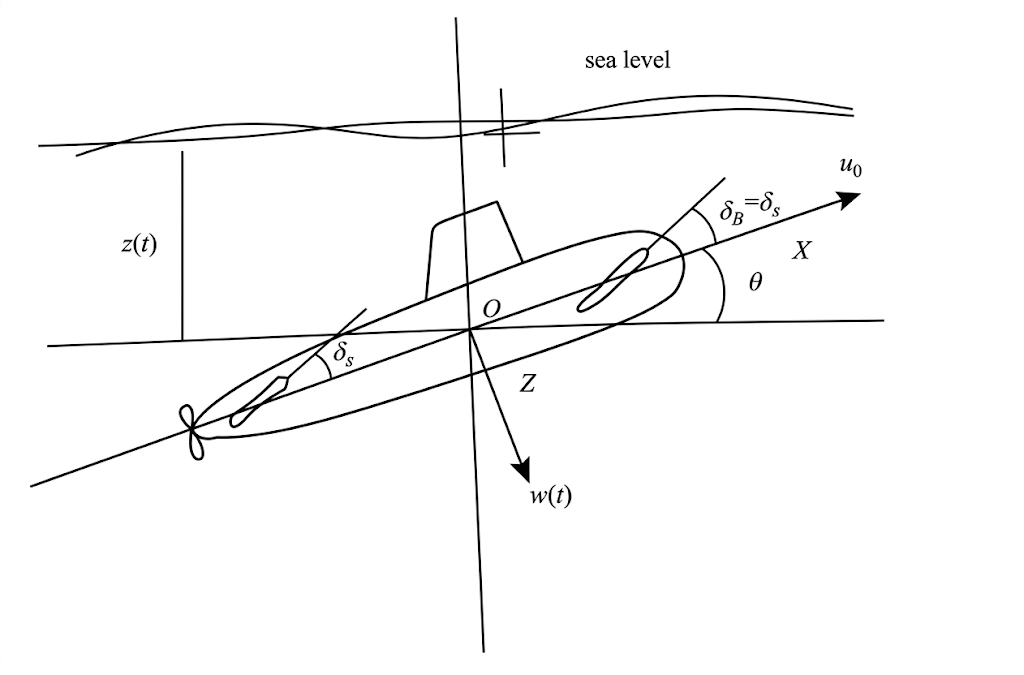
\includegraphics[width=0.75\linewidth]{a2_images/sub.png}
    \caption{Autopilot submarine}
    \label{fig:sub}
\end{figure}


\begin{enumerate}[resume]
    \item Determine the equilibrium point(s) of the submarine system when the control input is zero, i.e., $\delta_s = 0$. \hfill \textbf{[2 mark]}
    
    \begin{enumerate}[label=\alph*.]
        \item $\begin{bmatrix} w \\ q \end{bmatrix} = \begin{bmatrix} 0 \\ 0 \end{bmatrix}$
        \vspace{2mm}

        \item $\begin{bmatrix} w \\ q \end{bmatrix} = \begin{bmatrix} -0.04 \\ 0.002 \end{bmatrix}$
        \vspace{2mm}

        \item $\begin{bmatrix} w \\ q \end{bmatrix} = \begin{bmatrix} 0.02 \\ 0.002 \end{bmatrix}$
        \vspace{2mm}

        \item Infinite equilibrium points along the line $q = 0.04w$
        \vspace{2mm}

        \item None of the above.
    \end{enumerate}

    \item Using the state vector $\mathbf{x} = \begin{bmatrix} w \\ q \end{bmatrix}$ and input $u = \delta_s$, the state-space representation of the submarine dynamics is: \hfill \textbf{[4 marks]}
    
    \begin{enumerate}[label=\alph*.]
        \item $\dot{\mathbf{x}} = \begin{bmatrix} -0.04 & 1 \\ 0.002 & -0.1 \end{bmatrix}\mathbf{x} + \begin{bmatrix} -0.02 \\ -0.002 \end{bmatrix}u$
        \vspace{2mm}

        \item $\dot{\mathbf{x}} = \begin{bmatrix} -0.04 & 0.002 \\ 1 & -0.1 \end{bmatrix}\mathbf{x} + \begin{bmatrix} -0.02 \\ -0.002 \end{bmatrix}u$
        \vspace{2mm}

        \item $\dot{\mathbf{x}} = \begin{bmatrix} -0.04 & 1 \\ 0.002 & -0.1 \end{bmatrix}\mathbf{x} + \begin{bmatrix} 0.02 \\ 0.002 \end{bmatrix}u$
        \vspace{2mm}

        \item $\dot{\mathbf{x}} = \begin{bmatrix} 1 & -0.04 \\ -0.1 & 0.002 \end{bmatrix}\mathbf{x} + \begin{bmatrix} -0.02 \\ -0.002 \end{bmatrix}u$
        \vspace{2mm}

        \item None of the above.
    \end{enumerate}

    \item Determine the characteristic equation and the open-loop poles for the submarine system. What can be concluded about its stability? \hfill \textbf{[4 marks]}
    
    \begin{enumerate}[label=\alph*.]
        \item $s^2 + 0.14s + 0.002 = 0$; \quad $s \approx -0.0162, -0.1238$; \quad Stable
        \vspace{2mm}

        \item $s^2 + 0.14s + 0.006 = 0$; \quad $s \approx -0.07 \pm 0.0332j$; \quad Marginally stable
        \vspace{2mm}

        \item $s^2 - 0.14s + 0.002 = 0$; \quad $s \approx 0.0162, 0.1238$; \quad Unstable
        \vspace{2mm}

        \item $s^2 + 0.14s + 0.004 = 0$; \quad $s \approx -0.04, -0.10$; \quad Stable
        \vspace{2mm}

        \item None of the above.
    \end{enumerate}

    \item Design a full-state feedback controller $\mathbf{u} = -\mathbf{K}\mathbf{x}$ such that the closed-loop poles of the submarine are located at $s = -1\text{ rad/s}$ and $s = -0.5\text{ rad/s}$. The gain matrix $\mathbf{K}$ is: \hfill \textbf{[4 marks]}
    
    \begin{enumerate}[label=\alph*.]
        \item $\mathbf{K} = \begin{bmatrix} -148.71 & 807.14 \end{bmatrix}$
        \vspace{2mm}

        \item $\mathbf{K} = \begin{bmatrix} 148.71 & -807.14 \end{bmatrix}$
        \vspace{2mm}

        \item $\mathbf{K} = \begin{bmatrix} -68.00 & 807.14 \end{bmatrix}$
        \vspace{2mm}

        \item $\mathbf{K} = \begin{bmatrix} 807.14 & -148.71 \end{bmatrix}$
        \vspace{2mm}

        \item None of the above.
    \end{enumerate}
\end{enumerate}
    


\section{Question 2}
A quadcopter is a four-rotor helicopter. It is an under-actuated dynamic vehicle with four input forces and
associated drag moments (one for each rotor) and six Degrees Of Freedom (6DOF). The motion of a
quadcopter in 6DOF is controlled by varying the rpm of the four rotors individually, thereby changing the
thrust forces and rotational moments (from rotor drag). Roll (rotation about the x-axis) and pitch (rotation
about the y-axis) is controlled by changing the relative speed between pairs of opposite rotors. The rotors
rotate in clockwise- anticlockwise pairs as shown in Fig. \ref{fig:quad}. This pairing is exploited to control the yaw
moment (from the drag on the rotors) – it is possible to maintain overall net vertical thrust yet create a
yaw moment by running one opposite rotor pair (e.g. Rotor 1 and 3) faster than the other rotor pair (e.g.
Rotor 2 and 4). Sophisticated control is essential for a balance flight of quadcopter.

\begin{figure}[H]
    \centering
    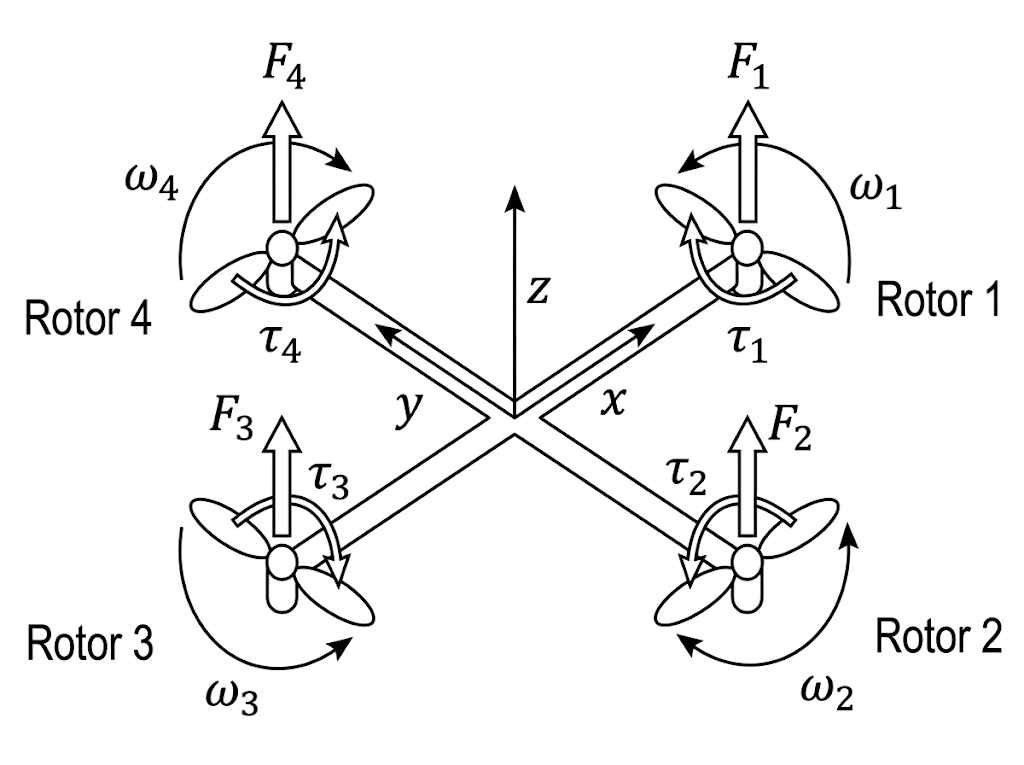
\includegraphics[width=0.75\linewidth]{a2_images/quadcopter.png}
    \caption{Enter Caption}
    \label{fig:quad}
\end{figure}

As a control engineer, your task now is to model the dynamics of a quadcopter and to design a sophisticated control system. To simplify the problem, only the heave (vertical) motion dynamics of the quadcopter is firstly considered, with its equation of motion given by
\begin{equation}
T = m\ddot{z} + b_z \dot{z} + mg
\end{equation}
where $T = F_1 + F_2 + F_3 + F_4$ is the total thrust force generated by the four rotors/propellers; $z$ is the vertical displacement of the quadcopter; $m$ is the total mass of the quadcopter; $b_z$ is the vertical aerodynamic drag coefficient; $g$ is acceleration of gravity. You may assume the following uses SI units.

\begin{enumerate}
    \item For the system described by Equation (1), and using the state variable $\mathbf{x} = \begin{bmatrix} z \\ \dot{z} \end{bmatrix}$ and input $\mathbf{u} = F_z = T - mg$, the state equation is given by: \hfill \textbf{[2 marks]}
    
    \begin{enumerate}[label=\alph*.]
        \item $\dot{\mathbf{x}} = \begin{bmatrix} 0 & 1 \\ 0 & -\frac{b_z}{m} \end{bmatrix} \mathbf{x} + \begin{bmatrix} 0 \\ \frac{1}{m} \end{bmatrix} \mathbf{u} \hfill (2)$
        \vspace{2mm}
        
        \item $\dot{\mathbf{x}} = \begin{bmatrix} 0 & 1 \\ 0 & -\frac{b_z}{m} \end{bmatrix} \mathbf{x} + \begin{bmatrix} 0 \\ -1 \end{bmatrix} \mathbf{u} \hfill (2)$
        \vspace{2mm}
        
        \item $\dot{\mathbf{x}} = \begin{bmatrix} -\frac{b_z}{m} & 0 \\ 1 & 0 \end{bmatrix} \mathbf{x} + \begin{bmatrix} \frac{1}{m} \\ 0 \end{bmatrix} \mathbf{u} \hfill (2)$
        \vspace{2mm}
        
        \item $\dot{\mathbf{x}} = \begin{bmatrix} -\frac{b_z}{m} & 0 \\ 1 & 0 \end{bmatrix} \mathbf{x} + \begin{bmatrix} -1 \\ 0 \end{bmatrix} \mathbf{u} \hfill (2)$
        \vspace{2mm}
        
        \item None of the above.
    \end{enumerate}

    \item For the state equation described by Equation (2), which statement below is \textbf{correct}? \hfill \textbf{[1 mark]}
    \begin{enumerate}[label=\alph*.]
        \item The state equation is in its minimal realisation.
        \item The system is in second order and thus has two poles.
        \item The system requires to be linearized around its equilibrium position.
        \item The determinant of A matrix is non-zero.
        \item None of the above.
    \end{enumerate}

    \vspace{0.5cm}

    \item Is the open loop system described by Equation (2) \hfill \textbf{[2 marks]}
    \begin{enumerate}[label=\alph*.]
        \item Stable?
        \item Marginally stable?
        \item Unstable?
        \item Conditionally stable?
        \item None of the above.
    \end{enumerate}

    \item Based on the pole locations, describe the dynamic behaviour of the open loop system. \hfill \textbf{[1 mark]}
    \begin{enumerate}[label=\alph*.]
        \item System will reach steady-state after long period of time.
        \item System will demonstrate oscillatory behaviour.
        \item System will demonstrate overshoot behaviour.
        \item System will exponentially converge to steady-state.
        \item None of the above.
    \end{enumerate}

    \vspace{0.5cm}

    \item For the system described by Equation (1), given that the states are $\begin{bmatrix} z \\ \dot{z} \end{bmatrix}$, input $\mathbf{u} = F_z = T - mg$, and the output is the vertical acceleration of the quadcopter, $\ddot{z}$, then the output equation is given by: \hfill \textbf{[2 marks]}
    
    \begin{enumerate}[label=\alph*.]
        \item $\mathbf{y} = \begin{bmatrix} 0 & 1 \\ 0 & -\frac{b_z}{m} \end{bmatrix} \mathbf{x} + \begin{bmatrix} 0 \\ \frac{1}{m} \end{bmatrix} \mathbf{u} \hfill (3)$
        \vspace{2mm}

        \item $\mathbf{y} = \begin{bmatrix} 0 & -\frac{b_z}{m} \end{bmatrix} \mathbf{x} + \frac{1}{m} \mathbf{u} \hfill (3)$
        \vspace{2mm}

        \item $\mathbf{y} = \begin{bmatrix} 1 & 0 \end{bmatrix} \mathbf{x} + 0\mathbf{u} \hfill (3)$
        \vspace{2mm}

        \item $\mathbf{y} = \begin{bmatrix} 0 & 1 \end{bmatrix} \mathbf{x} + 0\mathbf{u} \hfill (3)$
        \vspace{2mm}

        \item None of the above.
    \end{enumerate}

    \item Derive the transfer function between the total vertical input force, $F_z$ and the vertical velocity of the quadcopter, $\dot{z}$. The transfer function is given by: \hfill \textbf{[4 marks]}
    
    \begin{enumerate}[label=\alph*.]
        \item $\dfrac{1}{ms+b_z} \hfill (4)$
        \vspace{2mm}

        \item $\dfrac{1}{ms^2+b_z s} \hfill (4)$
        \vspace{2mm}

        \item $\dfrac{s}{ms^2+b_z s+mg} \hfill (4)$
        \vspace{2mm}

        \item $\dfrac{1}{ms^2+b_z s+mg} \hfill (4)$
        \vspace{2mm}

        \item None of the above.
    \end{enumerate}
\end{enumerate}

\vspace{0.5cm}

Now let's consider the coupled heave (vertical) and yaw ($z$-axis rotation) dynamic motions of the quadcopter. For the quadcopter to reach a torque balance on the roll ($x$-axis rotation) and pitch ($y$-axis rotation) axes, rotor 1 and rotor 3 are assumed to spin at the same speed and so do rotor 2 and rotor 4. The equations of motion are therefore given by
\begin{align}
2F_1 + 2F_2 &= m\ddot{z} + b_z \dot{z} + mg \\
2c(F_2 - F_1) &= I_z \ddot{\varphi} + b_{\varphi}\dot{\varphi}
\end{align}
where $F_1$ and $F_2$ are respectively the thrust force generated by rotor/propeller 1 and rotor/propeller 2; $c$ is the vertical thrust force to yaw torque scaling factor of each the rotor/propeller set (e.g. $\tau_1 = cF_1$); $I_z$ and $b_{\varphi}$ are respectively the moment of inertia and aerodynamic drag coefficient of the quadcopter yaw axis; and $\varphi$ is the yaw angle.

\begin{enumerate}[resume]
    \item For the dynamic system described by Equations (5) and (6), which statement below is \textbf{incorrect}? \hfill \textbf{[2 marks]}
    \begin{enumerate}[label=\alph*.]
        \item $mg$ is an uncontrollable input to the system.
        \item The system consists of two coupled mass-spring-damper sub-systems.
        \item The system has two controllable inputs.
        \item The system is marginally stable.
        \item None of the above.
    \end{enumerate}

    \vspace{0.5cm}

    \item For the dynamic system described by Equations (5) and (6), and using the state variable $\mathbf{x} = \begin{bmatrix} z \\ \dot{z} \\ \varphi \\ \dot{\varphi} \end{bmatrix}$ and control input $\mathbf{u} = \begin{bmatrix} F_1 \\ F_2 \end{bmatrix}$, the state equation is given by: \hfill \textbf{[4 marks]}
    \begin{enumerate}[label=\alph*.]
    \item $\dot{\mathbf{x}} = \begin{bmatrix} 0 & 1 & 0 & 0 \\ 0 & -\frac{b_z}{m} & 0 & 0 \\ 0 & 0 & 0 & 1 \\ 0 & 0 & 0 & -\frac{b_{\varphi}}{I_z} \end{bmatrix} \mathbf{x} + \begin{bmatrix} 0 & 0 \\ \frac{2}{m} & \frac{2}{m} \\ 0 & 0 \\ -\frac{2c}{I_z} & \frac{2c}{I_z} \end{bmatrix} \mathbf{u} + \begin{bmatrix} 0 \\ -1 \\ 0 \\ 0 \end{bmatrix} [g] \hfill (7)$
    \vspace{2mm}

    \item $\dot{\mathbf{x}} = \begin{bmatrix} 0 & 1 & 0 & 0 \\ 0 & -\frac{b_z}{m} & 0 & 0 \\ 0 & 0 & 0 & 1 \\ 0 & 0 & 0 & -\frac{b_{\varphi}}{I_z} \end{bmatrix} \mathbf{x} + \begin{bmatrix} 0 & 0 \\ \frac{2}{m} & \frac{2}{m} \\ 0 & 0 \\ \frac{2c}{I_z} & -\frac{2c}{I_z} \end{bmatrix} \mathbf{u} + \begin{bmatrix} 0 \\ -1 \\ 0 \\ 0 \end{bmatrix} [g] \hfill (7)$
    \vspace{2mm}

    \item $\dot{\mathbf{x}} = \begin{bmatrix} 0 & 1 & 0 & 0 \\ 0 & \frac{b_z}{m} & 0 & 0 \\ 0 & 0 & 0 & 1 \\ 0 & 0 & 0 & \frac{b_{\varphi}}{I_z} \end{bmatrix} \mathbf{x} + \begin{bmatrix} 0 & 0 \\ \frac{2}{m} & \frac{2}{m} \\ 0 & 0 \\ -\frac{2c}{I_z} & \frac{2c}{I_z} \end{bmatrix} \mathbf{u} + \begin{bmatrix} 0 \\ -1 \\ 0 \\ 0 \end{bmatrix} [g] \hfill (7)$
    \vspace{2mm}

    \item $\dot{\mathbf{x}} = \begin{bmatrix} 0 & 1 & 0 & 0 \\ 0 & \frac{b_z}{m} & 0 & 0 \\ 0 & 0 & 0 & 1 \\ 0 & 0 & 0 & \frac{b_{\varphi}}{I_z} \end{bmatrix} \mathbf{x} + \begin{bmatrix} 0 & 0 \\ \frac{2}{m} & \frac{2}{m} \\ 0 & 0 \\ \frac{2c}{I_z} & -\frac{2c}{I_z} \end{bmatrix} \mathbf{u} + \begin{bmatrix} 0 \\ -1 \\ 0 \\ 0 \end{bmatrix} [g] \hfill (7)$
    \vspace{2mm}

    \item None of the above.
    \end{enumerate}

    \item For the dynamic system described by Equations (5) and (6), and using the state variable $\mathbf{x} = \begin{bmatrix} z \\ \dot{z} \\ \varphi \\ \dot{\varphi} \end{bmatrix}$ and output $\mathbf{y} = \begin{bmatrix} z \\ \varphi \end{bmatrix}$, the output equation is given by: \hfill \textbf{[2 marks]}
    
    \begin{enumerate}[label=\alph*.]
        \item $\mathbf{y} = \begin{bmatrix} 0 & 1 & 0 & 0 \\ 0 & 0 & 0 & 1 \end{bmatrix} \mathbf{x} + \begin{bmatrix} 0 & 0 \\ 0 & 0 \end{bmatrix} \mathbf{u} + \begin{bmatrix} 0 \\ 0 \end{bmatrix} [g] \hfill (8)$
        \vspace{2mm}

        \item $\mathbf{y} = \begin{bmatrix} 0 & 0 & 0 & 0 \\ 0 & 1 & 0 & 0 \\ 0 & 0 & 0 & 0 \\ 0 & 0 & 0 & 1 \end{bmatrix} \mathbf{x} + \begin{bmatrix} 0 & 0 \\ 0 & 0 \\ 0 & 0 \\ 0 & 0 \end{bmatrix} \mathbf{u} + \begin{bmatrix} 0 \\ 0 \\ 0 \\ 0 \end{bmatrix} [g] \hfill (8)$
        \vspace{2mm}

        \item $\mathbf{y} = \begin{bmatrix} 1 & 0 & 0 & 0 \\ 0 & 0 & 1 & 0 \end{bmatrix} \mathbf{x} + \begin{bmatrix} 0 & 0 \\ 0 & 0 \end{bmatrix} \mathbf{u} + \begin{bmatrix} 0 \\ 0 \end{bmatrix} [g] \hfill (8)$
        \vspace{2mm}

        \item $\mathbf{y} = \begin{bmatrix} 0 & 1 & 0 & 1 \end{bmatrix} \mathbf{x} + \begin{bmatrix} 0 & 0 \end{bmatrix} \mathbf{u} + [0][g] \hfill (8)$
        \vspace{2mm}

        \item None of the above.
    \end{enumerate}

    \vspace{0.5cm}

    \item For the state space model described by Equations (7) and (8), determine the redundant states that can be removed from the model. \hfill \textbf{[2 marks]}
    
    \begin{enumerate}[label=\alph*.]
        \item $\begin{bmatrix} z \\ \dot{z} \end{bmatrix}$
        \vspace{2mm}

        \item $\begin{bmatrix} \varphi \\ \dot{\varphi} \end{bmatrix}$
        \item $\begin{bmatrix} \dot{z} \\ \dot{\varphi} \end{bmatrix}$
        \vspace{2mm}

        \item $\begin{bmatrix} z \\ \varphi \end{bmatrix}$
        \vspace{2mm}

        \item None of the above.
    \end{enumerate}

    \vspace{0.5cm}

    \item Consider the dynamic system described by Equations (5) and (6). If the controllability matrix is full rank, how many states are controllable? \hfill \textbf{[1 mark]}
    \begin{enumerate}[label=\alph*.]
        \item One
        \item Two
        \item Four
        \item Six
        \item None of the above.
    \end{enumerate}
\end{enumerate}

Now let's consider the coupled roll ($x$-axis rotation) and sway ($y$-axis translation) motions of the quadcopter. In this case, rotor 2 and rotor 4 are no longer spinning at the same speed in order to roll. The simplified and linearized dynamics of the system can be written as the following state space form:

\begin{equation}
\dot{\mathbf{x}} = \begin{bmatrix} 
0 & 1 & g & 0 \\ 
0 & -\dfrac{b_y}{m} & 0 & 0 \\ 
0 & 0 & 0 & 1 \\ 
0 & 0 & 0 & -\dfrac{b_\theta}{I_x} 
\end{bmatrix} \mathbf{x} + 
\begin{bmatrix} 
0 & 0 \\ 
0 & 0 \\ 
0 & 0 \\ 
-\dfrac{a}{I_x} & \dfrac{a}{I_x} 
\end{bmatrix} \mathbf{u}
\end{equation}

\begin{equation}
\mathbf{y} = \begin{bmatrix} 
0 & 1 & 0 & 0 \\ 
0 & 0 & 0 & 1 
\end{bmatrix} \mathbf{x} + 
\begin{bmatrix} 
0 & 0 \\ 
0 & 0 
\end{bmatrix} \mathbf{u}
\end{equation}

where $\mathbf{x} = \begin{bmatrix} y \\ \dot{y} \\ \theta \\ \dot{\theta} \end{bmatrix}$, $\mathbf{u} = \begin{bmatrix} F_2 \\ F_4 \end{bmatrix}$, $\mathbf{y} = \begin{bmatrix} \dot{y} \\ \dot{\theta} \end{bmatrix}$; $b_y$ is the aerodynamic drag coefficient of the quadcopter sway axis; $I_x$ and $b_\theta$ are respectively the moment of inertia and aerodynamic drag coefficient of the quadcopter roll axis; $\theta$ is the roll angle; and $a$ is the lever arm -- the distance between the rotor centre of rotation and the quadcopter centre of rotation.

\begin{enumerate}[resume]
    \item For the state space model described by Equations (9) and (10), which statement below is \textbf{correct}? \hfill \textbf{[2 marks]}
    \begin{enumerate}[label=\alph*.]
        \item The model is accurate for control only when the quadcopter rotates in small roll angles.
        \item Full state feedback control can be directly applied to the system without the design of an observer.
        \item The controllability matrix is a 4x4 matrix.
        \item Full state feedback control is only able to add in additional damping but not stiffness.
    \end{enumerate}
\end{enumerate}

Now your task is to design a controller for roll ($x$-axis rotation) motion dynamics only and use an Inertia Measurement Unit (IMU) to measure the roll velocity as the system output, Equations (9) and (10) can be reduced to the following form:

\begin{equation}
\dot{\mathbf{x}} = \begin{bmatrix} 0 & 1 \\ 0 & -\frac{b_\theta}{I_x} \end{bmatrix} \mathbf{x} + \begin{bmatrix} 0 & 0 \\ -\frac{a}{I_x} & \frac{a}{I_x} \end{bmatrix} \mathbf{u}
\end{equation}

\begin{equation}
\mathbf{y} = \begin{bmatrix} 0 & 1 \end{bmatrix} \mathbf{x} + \begin{bmatrix} 0 & 0 \end{bmatrix} \mathbf{u}
\end{equation}

where $\mathbf{x} = \begin{bmatrix} \theta \\ \dot{\theta} \end{bmatrix}$, $\mathbf{u} = \begin{bmatrix} F_2 \\ F_4 \end{bmatrix}$, $\mathbf{y} = [\dot{\theta}]$.

\vspace{0.5cm}

\begin{enumerate}[resume]
    \item For the state space model described by Equations (11) and (12), you are going to design a full state feedback controller that is able to place the closed loop poles of the system at the desired locations to achieve a 2\% settling time of 2s and an overshoot of 15\%. What should the locations of the poles be? 
    \textbf{[2 marks]}
    \begin{enumerate}[label=\alph*.]
        \item $s = -2 \pm 2j\text{ rad/s}$
        \item $s = -2 \pm 3.312j\text{ rad/s}$
        \item $s = 2 \pm 3.312j\text{ rad/s}$
        \item $s = -4 \pm 2j\text{ rad/s}$
        \item None of the above.
    \end{enumerate}
    \item You decide instead that you want a more aggressive controller with a 2\% settling time of 1s and an overshoot of 10\%[cite: 13]. The required poles for these performance specifications are $s = -4 \pm 5.46j\text{ rad/s}$. Using pole placement, calculate the gain matrix $\mathbf{K}$ to position the closed loop poles at the desired location[cite: 13]. Asssume $I_x = 0.02\text{ kg}\cdot\text{m}^2$, $a = 0.15\text{m}$, and $b_\theta$ is approximated as zero for this question[cite: 13]. Hint: You have Rotor 2 and Rotor 4 generating moments in opposite directions about the roll axis, and thus you can assume $\mathbf{K} = \begin{bmatrix} -k_1 & -k_2 \\ k_1 & k_2 \end{bmatrix}$ in calculation. \hfill \textbf{[4 marks]}
    
    \begin{enumerate}[label=\alph*.]
        \item $\mathbf{K} = \begin{bmatrix} -0.5333 & -3.0541 \\ 0.5333 & 3.0541 \end{bmatrix}$
        \vspace{2mm}

        \item $\mathbf{K} = \begin{bmatrix} -1.5333 & -3.0541 \\ 1.5333 & 3.0541 \end{bmatrix}$
        \vspace{2mm}

        \item $\mathbf{K} = \begin{bmatrix} -3.0541 & -0.5333 \\ 3.0541 & 0.5333 \end{bmatrix}$
        \vspace{2mm}

        \item $\mathbf{K} = \begin{bmatrix} -3.0541 & -1.5333 \\ 3.0541 & 1.5333 \end{bmatrix}$
        \vspace{2mm}

        \item None of the above.
    \end{enumerate}
    
\end{enumerate}

\section{Question 3}
\begin{enumerate}
    \item   With reference to the bike schematic shown in Fig. \ref{fig:bike} , consider the relationship from steering angle $\delta$ to tilt angle $\varphi$. From your knowledge of bicycles, how would you describe this relationship? \textbf{[1 marks]}
\begin{figure}
    \centering
    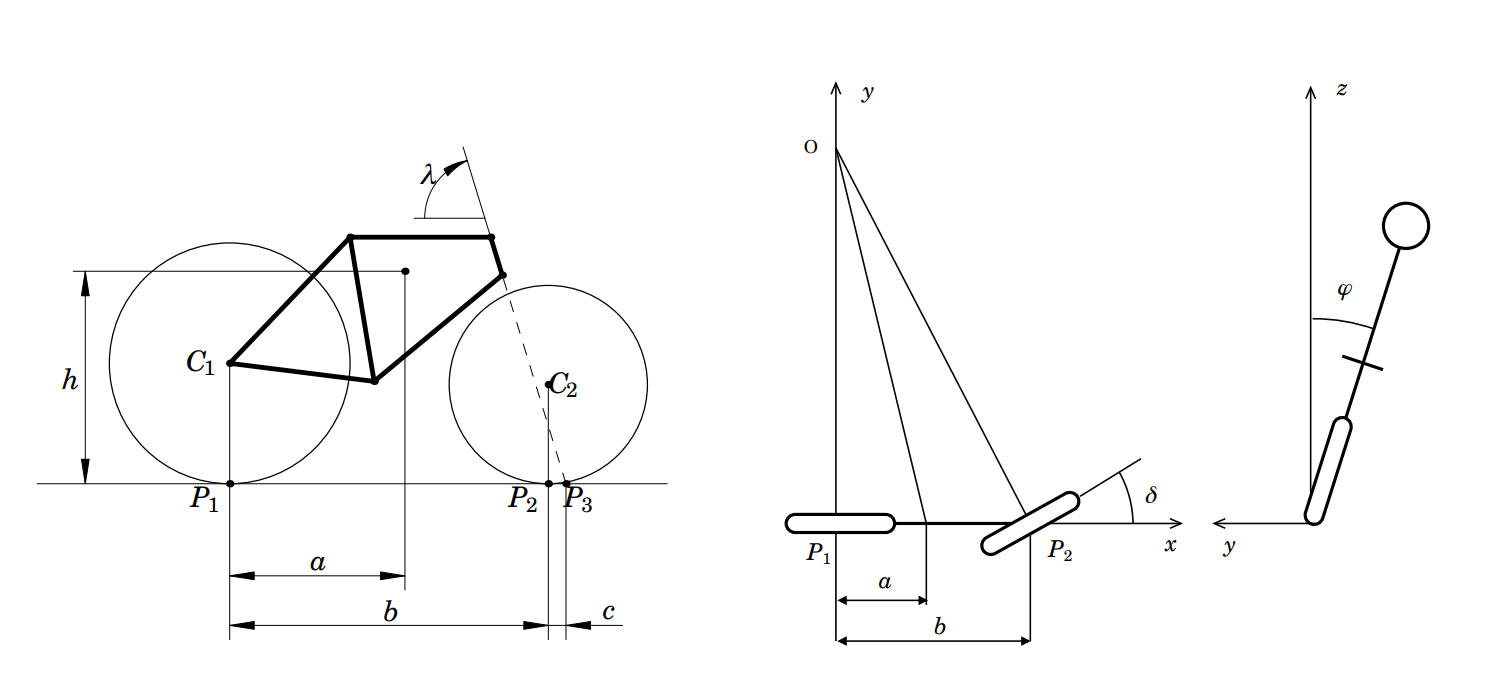
\includegraphics[width=0.75\linewidth]{a2_images/bicycle.PNG}
    \caption{Schematic of a bike (left: side view; centre: top view; right: front view)}
    \label{fig:bike}
\end{figure}
    \begin{enumerate}
        \item  {Stable}
        \item  \textbf{{Unstable}}
        \item  {Marginally stable}
        \item  {Non-minimum phase}
        \item  {None of the above.}
    \end{enumerate}
\end{enumerate}

After linearisation, the dynamic equation relating steering angle $\delta$ to tilt angle $\varphi$ is
\newcommand\dd[3][]{\frac{d#1#2}{d#3#1}}
\[
  \label{eq:bikedyn}
  \dd[^2]{\varphi}{t} = \frac{mgl}{J}\varphi + \frac{mlV_0^2}{bJ}\delta + \frac{amlV_0}{bJ}\dd{\delta}{t} \,.
\]
Most constants are unimportant and can be inferred. They can assumed to be all positive. $V_0$ is velocity. Ignoring many things, the relationship of the front fork with input torque~$T$ on the behaviour of the bike can be expressed as
\[
  T - mgt\varphi -mgt\alpha\delta = 0 \,.
\]
Or more simply, with trivial substitutions:
\[
  \delta = -k_1\varphi +k_2T \,.\label{eq:fork}
\]

\begin{enumerate}[resume]
    \item What is the transfer function from $\delta(s)$ to $\varphi(s)$? \textbf{[2 marks]}


    \begin{enumerate}
        \item {$\displaystyle P(s) = \frac{bJ}{amlV_0}\frac{s^2-mgl/J}{s+V_0/a} $}
        \item \textbf{{$\displaystyle P(s) = \frac{amlV_0}{bJ}\frac{s+V_0/a}{s^2-mgl/J} $}}
        \item {$\displaystyle P(s) = \frac{amlV_0}{bJ}\frac{s+V_0/a}{s^2+mgl/J} $}
        \item {None of the above.} 
    \end{enumerate}

    \item Combine Eqs~\eqref{eq:bikedyn} and \eqref{eq:fork} to write the dynamic equation of the system as a separated ODE in terms of tilt angle $\varphi$ to handlebar torque $T$. This equation is which of the following? \textbf{[3 marks]}

    \begin{enumerate}
        \item $\displaystyle 
          \ddot\varphi + \frac{amlk_1V_0}{bJ}\dot\varphi + \frac{mgl}{J}\biggl(\frac{k_1V_0^2}{bg}+1\biggr)\varphi= \frac{amk_2lV_0}{bJ}\biggl(\dot T + \frac{V_0}{a}T\biggr)
          $
        
        \item $\displaystyle 
          m\ddot\varphi - \frac{alk_1V_0}{bJ}\dot\varphi + \frac{gl}{J}\biggl(\frac{k_1V_0^2}{bg}-1\biggr)\varphi= \frac{ak_2lV_0}{bJ}\biggl(\dot T - \frac{V_0}{a}T\biggr)
          $
        
        \item $\displaystyle 
          m\ddot\varphi - \frac{alk_1V_0}{bJ}\dot\varphi + \frac{gl}{J}\biggl(\frac{k_1V_0^2}{bg}+1\biggr)\varphi= \frac{ak_2lV_0}{bJ}\biggl(\dot T - \frac{V_0}{a}T\biggr)
          $
            
        \item \textbf{$\displaystyle 
          \ddot\varphi + \frac{amlk_1V_0}{bJ}\dot\varphi + \frac{mgl}{J}\biggl(\frac{k_1V_0^2}{bg}-1\biggr)\varphi= \frac{amk_2lV_0}{bJ}\biggl(\dot T + \frac{V_0}{a}T\biggr)
          $}
        \item{None of the above.}
    \end{enumerate}

    \item Under what conditions is the torque-to-tilt system stable?\textbf{[3 marks]}
    
    \begin{enumerate}
        \item \textbf{{$V_0^2>bg/k_1$}}
        \item {$V_0^2<bg/k_1$}
        \item {$V_0/a<0$}
        \item {$V_0/a>0$}
        \item {Always}
        \item {Never}
        \item {None of the above.}
    \end{enumerate}
    

    \item It has been suggested that a bicycle with rear-wheel steering could have a mechanically-easier transmission design. The transfer function in this case would be:
        \[
          \frac{\varphi(s)}{\delta(s)} = \frac{\frac{mlV_0^2}{bJ} + \frac{amlV_0}{bJ}s}{s^2 - \frac{mgl}{J}}
          = \frac{mlV_0}{bJ}\frac{{V_0} - {a}s}{s^2 - mgl/J}
        \]
    Comment on the difficulty of control for this system compared to the bicycle with front-wheel steering.
    \textbf{[2 marks]}
        \begin{enumerate}
            \item {Easier to control.}
            \textbf{\item {Harder to control.}}
            \item {Neither easier nor harder to control.}
        \end{enumerate}

    \item The state, $A$, and $B$ matrices for this system are:
        \[
        x=\begin{bmatrix}
        \dot \varphi \\
        \dot \delta \\
        \varphi \\
        \delta
        \end{bmatrix}\qquad
        A=\begin{bmatrix}
        0 & 1 & 9 & 6 \\
        -7 & -5 & -15 & 76 \\
        1 & 0 & 0 & 0 \\
        0 & 1 & 0 & 0   
        \end{bmatrix}\qquad
        B = \begin{bmatrix}
        0 \\ 8 \\ 0 \\ 0
        \end{bmatrix}
        \]
    The characteristic equation to solve for the poles of this system is which of the following? \textbf{[3 marks]}
    \begin{enumerate}
        
        \textbf{\item {$\polynomial[reciprocal,var=s]{1,5,-78,12,774}=0$}}
        \item {$\polynomial[reciprocal,var=s]{1,-5,-78,12,774}=0$}
        \item {$\polynomial[reciprocal,var=s]{1,-5,78,-12,774}=0$}
        \item {$\polynomial[reciprocal,var=s]{5,-60,-47,774}=0$}
        \item {None of the above.}
    \end{enumerate}

    \item The poles of this system are which of the following? \textbf{[2 marks]}
        \begin{enumerate}
            \item {$s = -11.4 \qquad s = -3.0 \qquad s = 4.7$}
            \item {$s = -11.4 \qquad s = \phantom{-}3.0 \qquad s = 4.7$}
            \item {$s = \phantom{-}11.4 \qquad s = -3.0 \qquad s = 4.7\pm1.0i$}
            \textbf{\item {$s = -11.4 \qquad s = -3.0 \qquad s = 4.7\pm1.0i$}{}}
            \item{None of the above.}
        \end{enumerate}

    \item Which  of the following corresponds to the controllability matrix? \textbf{[4 marks]}

        \begin{enumerate}
        \item {\small$\begin{bmatrix}
        0 & 8 & 8 & -584 \\
        8 & -40 & 752 & 6976 \\
        0 & 0 & 8 & 8 \\
        0 & 8 & -40 & 752   
        \end{bmatrix}$}
        \item {\small$\begin{bmatrix}
        0 & 8 & 8 & -696 \\
        8 & -40 & 864 & 7536 \\
        0 & 0 & 8 & 8 \\
        0 & 8 & -40 & 864   
        \end{bmatrix}$}
        \textbf{\item {\small$\begin{bmatrix}
        0 & 8 & 8 & 584 \\
        8 & -40 & 752 & -6976 \\
        0 & 0 & 8 & 8 \\
        0 & 8 & -40 & 752   
        \end{bmatrix}$}{}}
        \item {\small$\begin{bmatrix}
        0 & 8 & 8 & 696 \\
        8 & -40 & 864 & -7536 \\
        0 & 0 & 8 & 8 \\
        0 & 8 & -40 & 864   
        \end{bmatrix}$}
        \end{enumerate}
    \end{enumerate}


    \textbf{The rest of the question uses pole placement and LQR, need to check with Will whether to continue include the rest, or maybe try to come up with some frequency analysis questions}
\end{document}
